\section{The H tagging and W/Z tagging algorithms}
\label{sec: H tagging}

The products of hadronic decays of Higgs, W, and Z bosons can fall
within a single jet if these particles are highly boosted.  In this
analysis, we aim to cover as much of the Higgs branching ratio as
possible.  The Standard Model Higgs with a mass of 125 \GeVcc decays
to b$\bar{\rm b}$ with a branching fraction of 57.7\%, and to WW$^*$
with a braching fraction of 21.4\%.~\cite{pdg-higgs}.  Using these two
decay modes in a VH search, where WW$^*$ specifically decays to four
quarks, is the main topic of this note.  (The semileptonic decay mode
$ H \to WW \to 2q\ell \nu$ is viable, but its reconstruction is more
involved and will be covered in a subsequent analysis.)

%% &&& {\bf TO-DO: consider adding the branching fraction plot here. }


The algorithms to identify W/Z, ${\rm H \to b\bar{b}}$ and 
${\rm H \to WW^*}$ jets are necessarily different, but they use similar
jet-level variables: N-subjettiness (described in
Section~\ref{sec:N-subjettiness}) and jet pruning
(Section~\ref{sec:jetPruning}).  The W/Z-tagger is described in
Section~\ref{sec:wztagging}, and the two H-taggers in
Sections~\ref{sec:higgsTaggerbb} and ~\ref{sec:higgsTaggerww}.


%{\bf TO-DO: add a plot of this Higgs jet mass from signal, QCD, data, as a comparison.  And we need also to show the optimization of this mass choice. }

\subsection{N-subjettiness}
\label{sec:N-subjettiness}

N-subjettiness~\cite{Thaler:2010tr,Thaler:2011gf,Stewart:2010tn}
exploits the fact that the pattern of the hadronic decay of a heavy
object is reflected through the presence of distinctive energy lobes
corresponding to the decay products, as opposed to QCD jets which
present a more uniformly spread energy configuration. 
The inclusive jet shape N-subjettiness is
defined, in its generalized version~\cite{Thaler:2010tr}, as
%
\begin{equation}
\tau_N = \frac{1}{d_{0}} \sum_{k} p_{T,k}\,min( (\Delta R_{1,k})^{\beta}, (\Delta R_{2,k})^{\beta}...(\Delta R_{N,k})^{\beta})
\end{equation}
%
where the index $k$ runs over the jet constituents and the distances
$\Delta R_{n,k}$ are calculated with respect to the axis of the $n^{\mathrm{th}}$
subjet. The normalization factor $d_{0}$ is calculated as $d_{0}=
\sum_{k} p_{T,k}R^{\beta}_{0}$, setting $R_{0}$ to the jet radius of
the original jet. In the analysis, we use onepass\_kt\_axes definition
of subjet axes and the N-subjettiness is calculated
from the unpruned jets with the parameter $\beta=1$. 
It has been shown in the literature~\cite{Thaler:2010tr} that the
best way to separate (N+1)-prong from the N-prong decays merged into
a single jet is to select jets with low value of the ratio $\tau_{N+1}/\tau_N$.
In this vein, the variable able to best discriminate between $\PW/\cPZ$ jets and QCD jets
is $\tau_{21}=\tau_{2} / \tau_{1}$. The distribution of $\tau_{21}$ for
the VV signal and QCD background is given in Fig.~\ref{fig:N-sub-mass}.
%While, 
%the best variable to discriminate $H \to WW$ is $\tau_{42}=\tau_{4} / \tau_{2}$, given in 
%Fig.~\ref{fig:tau421TeV} and Fig.~\ref{fig:tau422TeV}.

\begin{figure}[htb]
\centering
\begin{tabular}{cc}
     \resizebox{0.5\linewidth}{!}{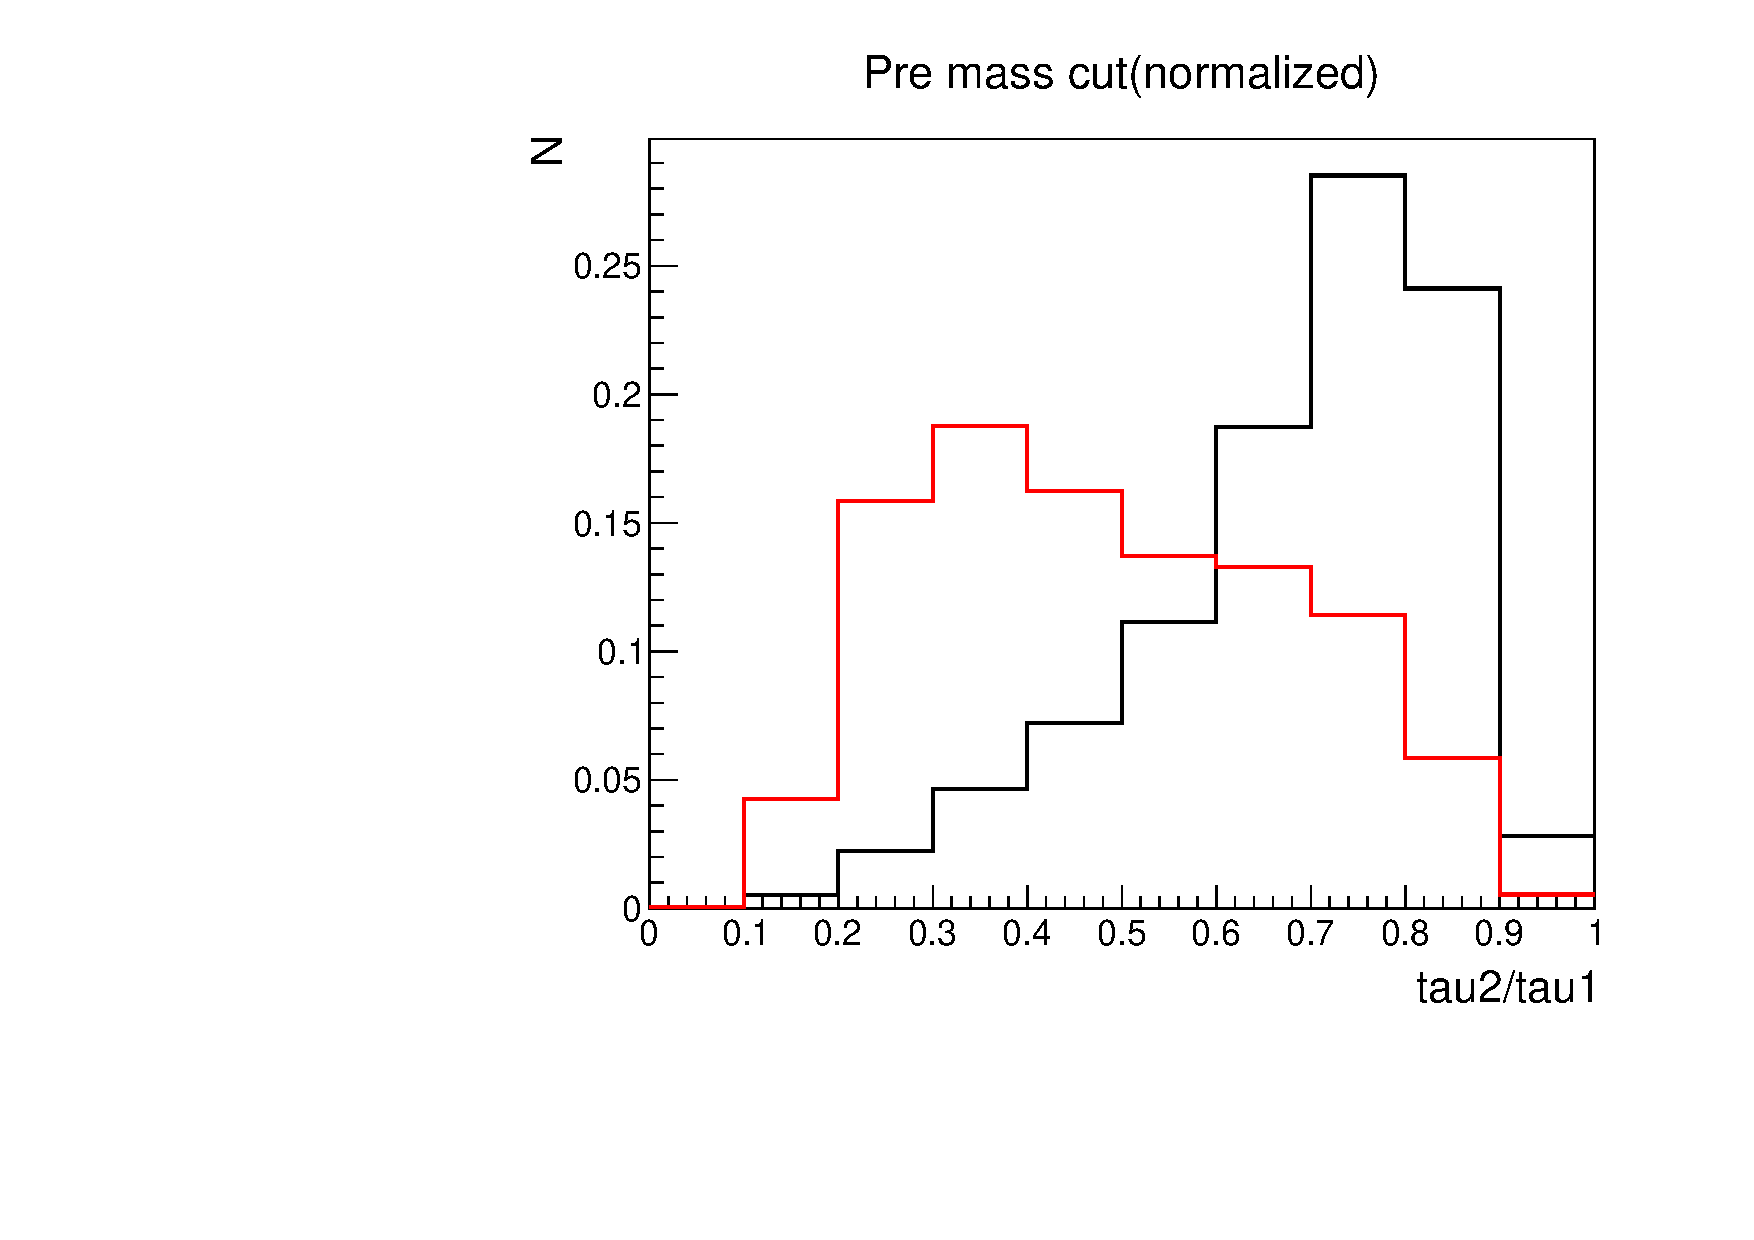
\includegraphics{EXO-14-009/figs/N-subjettiness/Signal_MC_Pre.pdf}} &
     \resizebox{0.5\linewidth}{!}{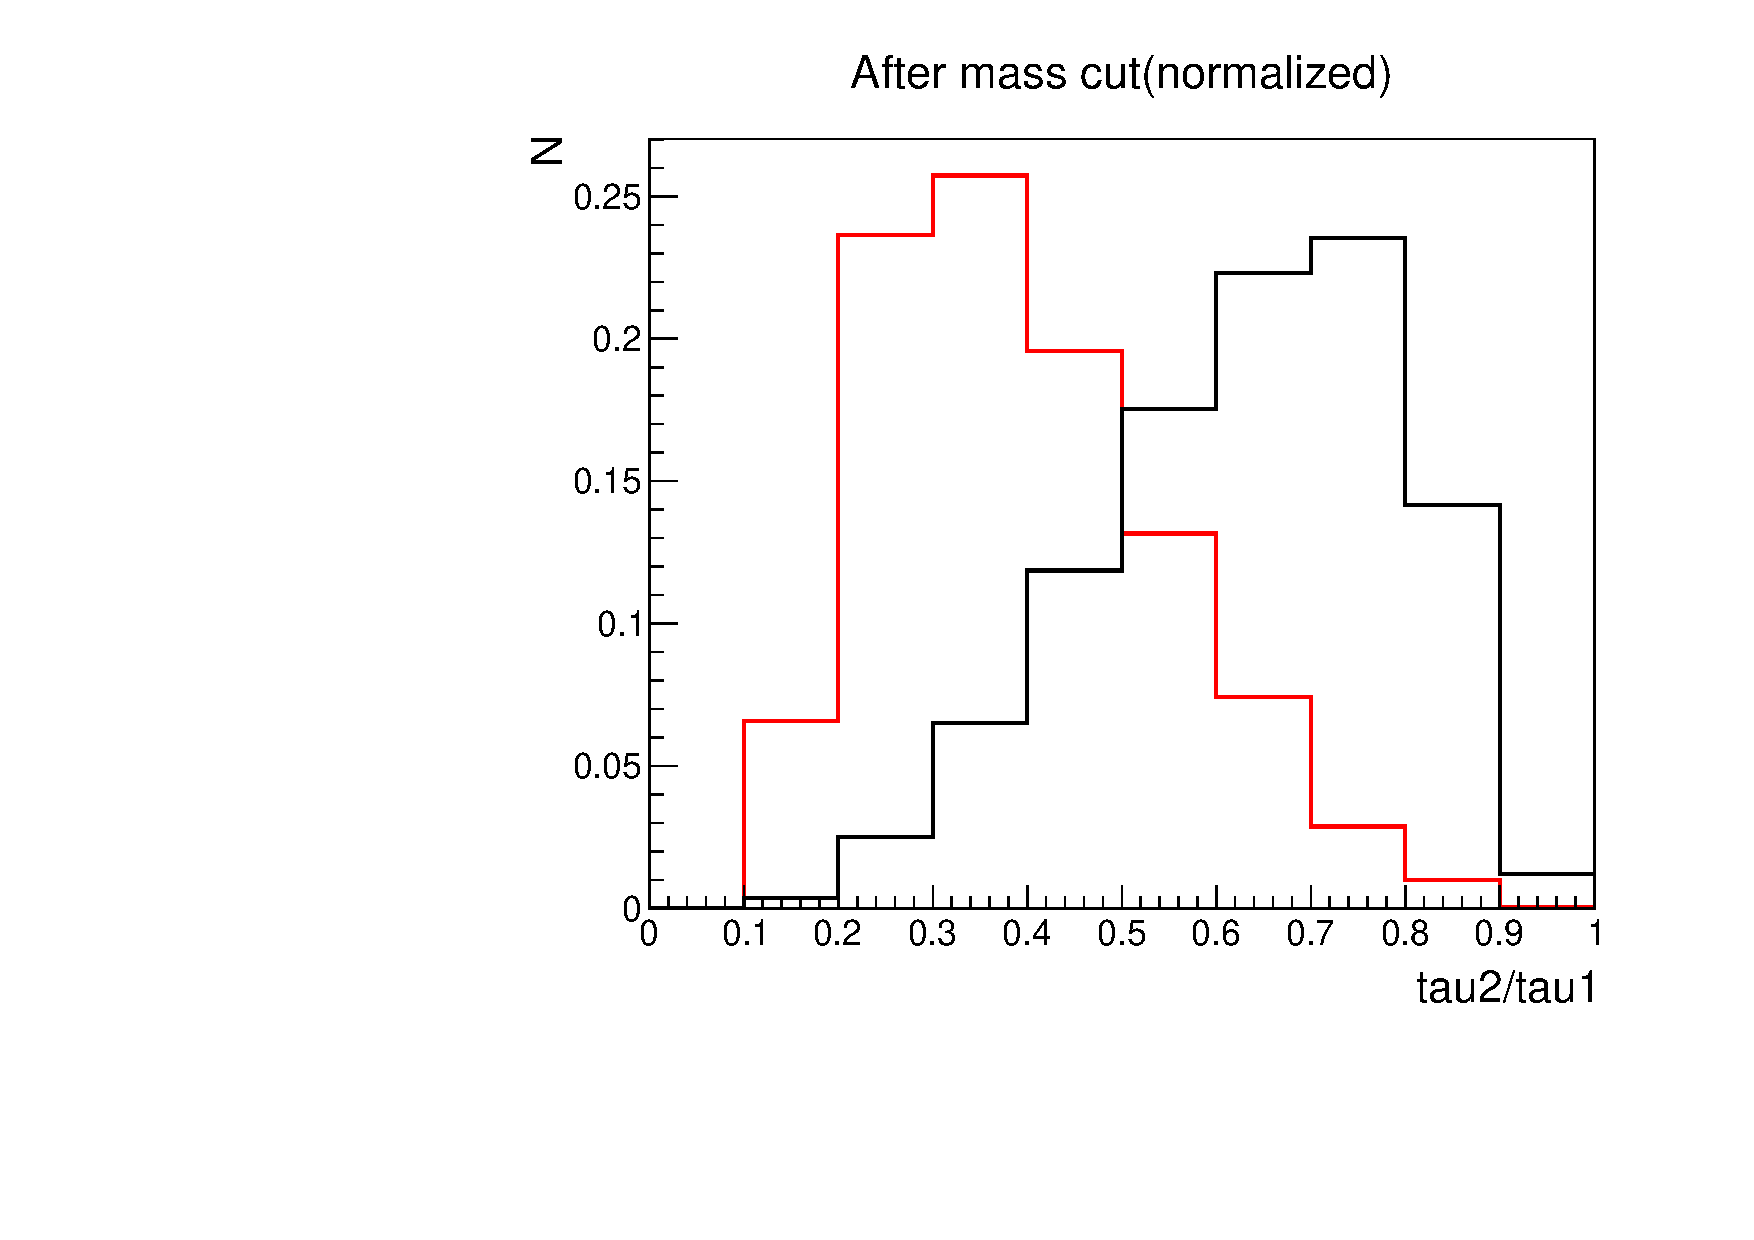
\includegraphics{EXO-14-009/figs/N-subjettiness/Signal_MC.pdf}} \\
\end{tabular}
\caption[N-subjettiness]{Comparison for $\tau_{2}/\tau_{1}$ distribution 
between signal (red) and background (black) 
before the jet mass cut (left) and after 
the jet mass cut of [70, 100]~GeV applied (right). 
The signal MC used here is Herwig WW 1.5 TeV, and background is Herwig QCD.}
\label{fig:N-sub-mass}
\end{figure}

%\textbf{PLAN} in Fig~\ref{N-sub} and Fig~\ref{N-sub-mass}, I'm gonna add prettier plots for different signals(pythia and herwig, 1.0Tev to 3.0TeV resonance).  

%The leading two ungroomed CA8 jets to the leading two pruned CA8 jets are matched requireing $\Delta R < 0.5 $, which fails in less than 0.1\% of the events.




\subsection{Jet Pruning}
\label{sec:jetPruning}

Jet pruning consists of the removal of the softest
components of the jets~\cite{catop_cms,topwtag_pas}.
The jet pruning algorithm uses the CA $R=0.8$ jets as inputs. In the
process, soft and wide-angle particles (relative to the parent in the
clustering) are ignored and are not clustered.  
The same parameters are chosen for the jet
pruning algorithm as in the original paper~\cite{jetpruning1,jetpruning2}.

%% &&& from Petar: is this really true?  I thought that the pruning
%% &&& reruns the CA8 jet clustering from scratch, but in the process
%% &&& prunes the soft and wide-angle PF candidates from the jet.
%% &&& We should check this...


The result of jet pruning on the CA8 jets is two fold, i.e., the invariant jet mass 
reconstruction and subjet indentification.
In all cases,
we use the jet invariant mass computed from the whole (or ``fat'') 
pruned jet.  This quantity is referred below to as the pruned jet mass.
For W/Z tagging, we use pruned jet mass between 70 and 100 \GeVcc. 
%is sychorinzed with VV search~\cite{EXO-12-024}.
For the identification of Higgs jets, we require the pruned jet mass to
lie between 110 and 135~\GeVcc.  The distribution of the pruned jet
mass of the Higgs candidate jet is shown on Fig.~\ref{fig:JetMassTagging} 


\begin{figure}[htb]
\begin{center}
%\includegraphics[width=0.49\textwidth]{HbbZqqfigs/Signal/signal-data-qcd-jetmass.pdf}
%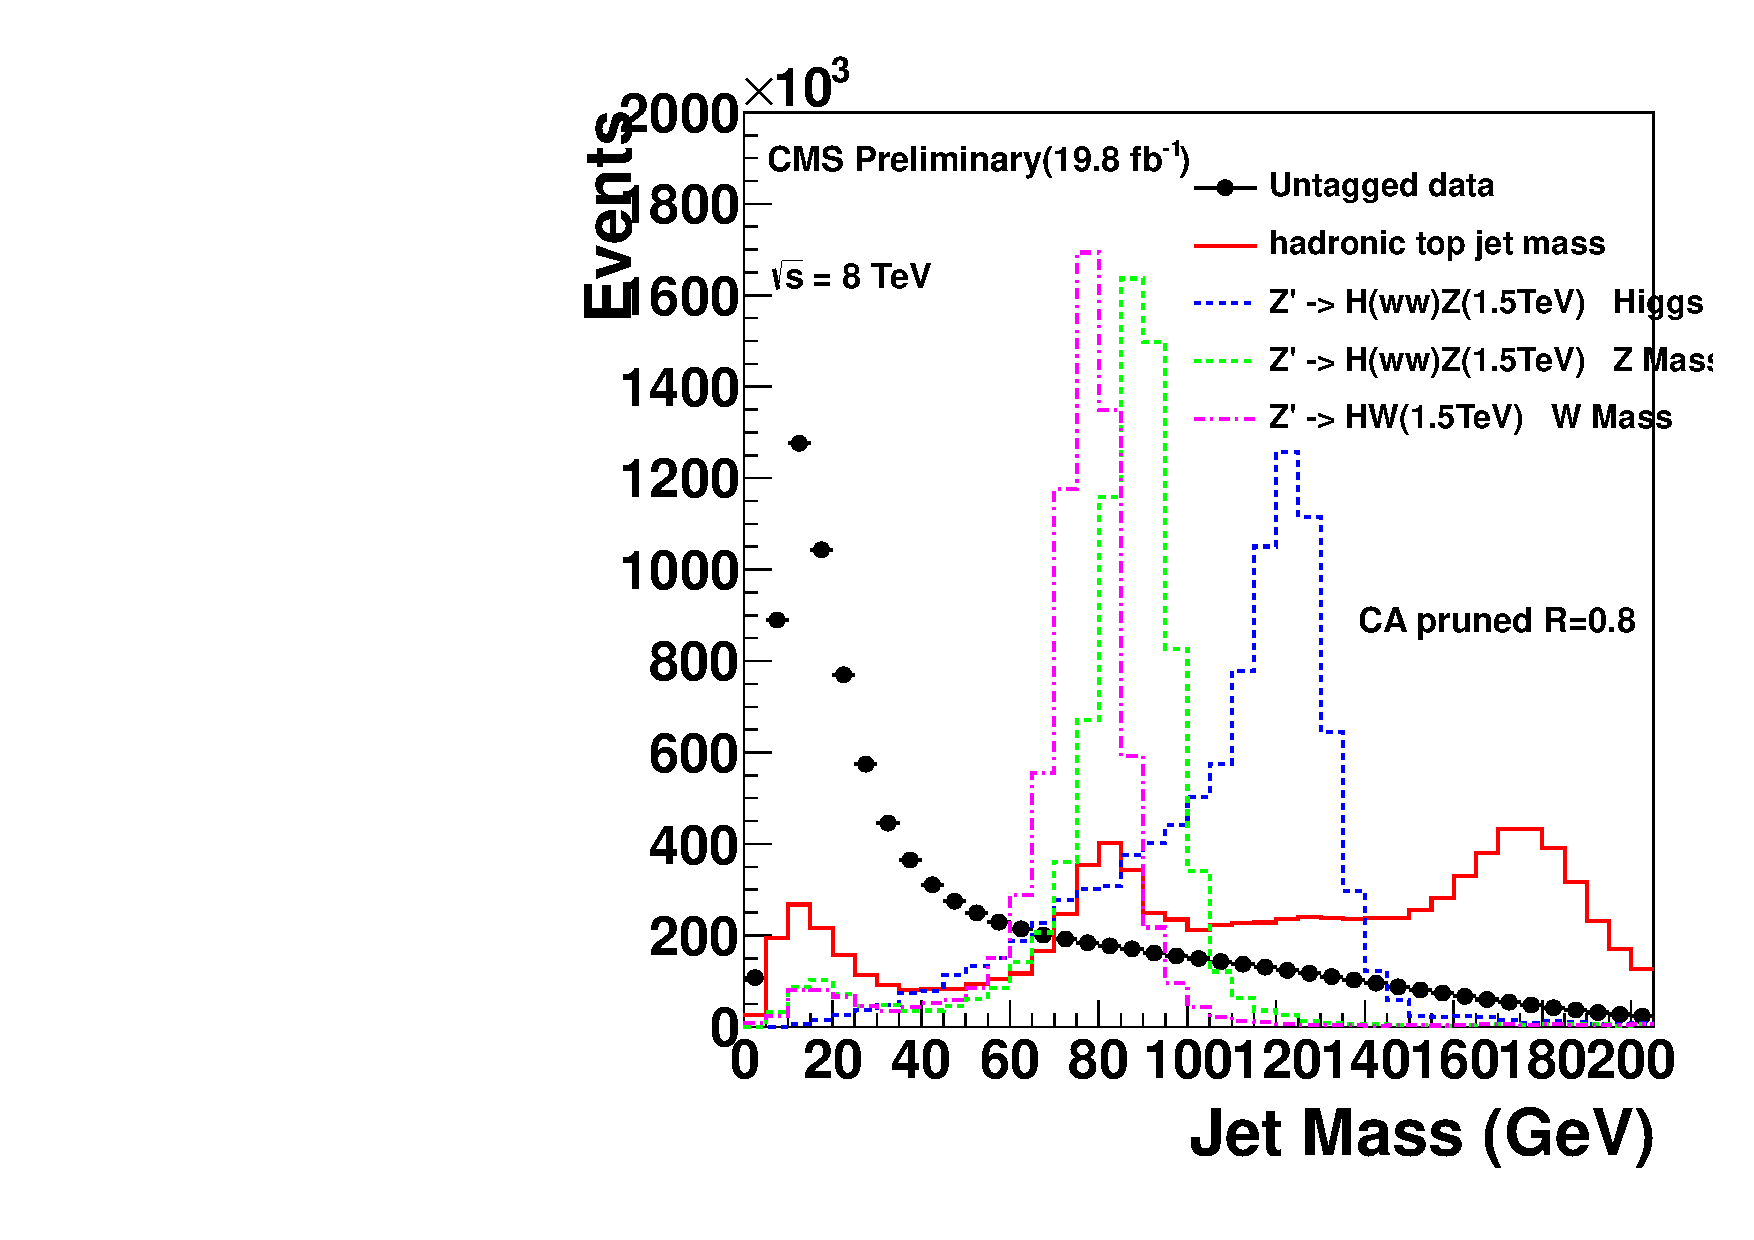
\includegraphics[width=0.49\textwidth]{HqqqqZqqfigs/Signal/signal-data-qcd-jetmass.pdf}
%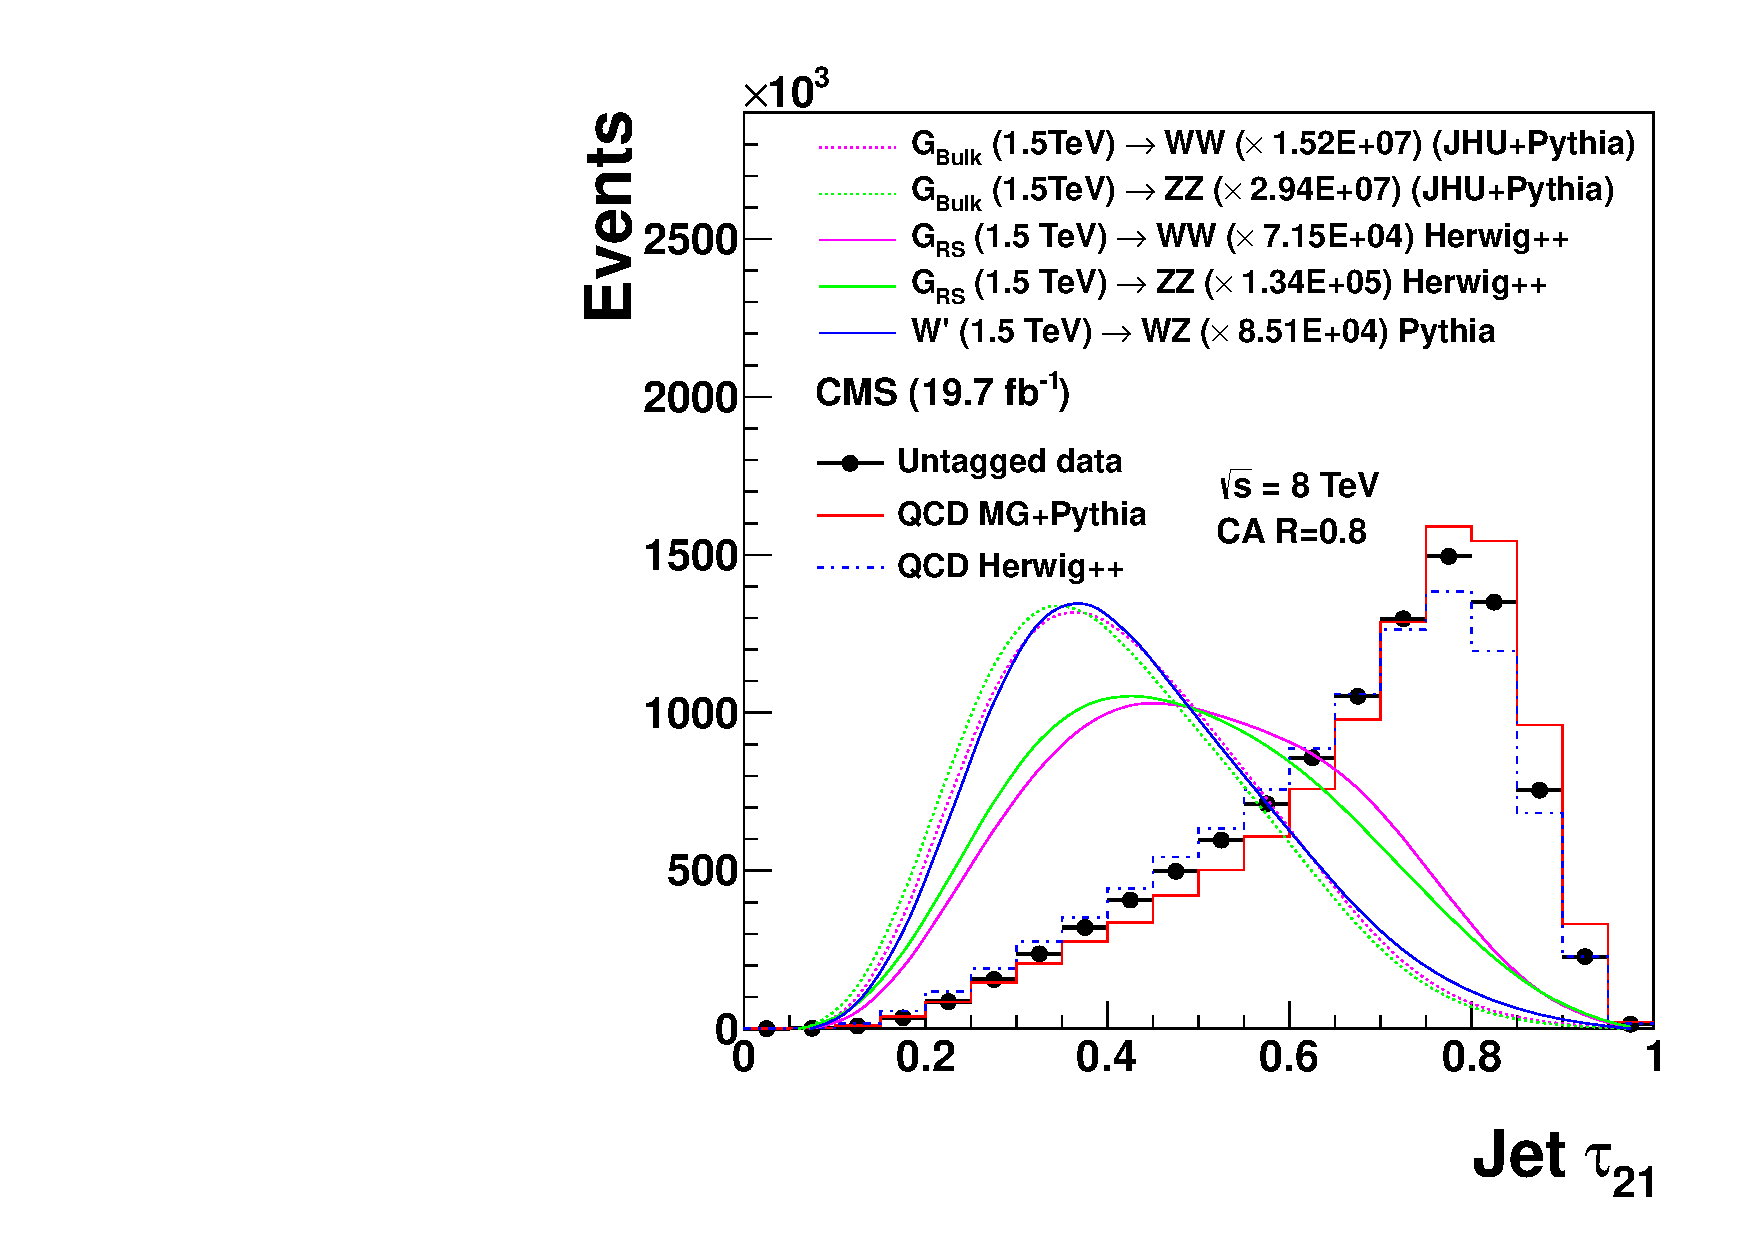
\includegraphics[width=0.49\textwidth]{figs/signal-acc-eff/signal-data-qcd-Jet-Tau21.pdf}
\includegraphics[width=0.69\textwidth]{EXO-14-009/HbbZqqfigs/Signal/signal-data-qcd-jetmass.pdf}
\end{center}
\caption{Pruned jet mass in signal MC, data and $t\overline{t}$ MC. 
  MC samples are normalized to data.  MC
  distributions are plotted as smooth curves connecting the histogram
  entries; the MC histograms have the same binning as the data.
  Higgs, W/Z and top jets are matched to their generator level particles, 
  respectively. }
%The pruned jet mass of $\Hbb$ jets is shown on
%  the left, and of $\Hww$ jets on the right.}
%  MC is normalized to fit into the plot.  }
 % The signal MC
 % distributions are plotted as smooth curves connecting the histogram
  %entries. 
\label{fig:JetMassTagging}
\end{figure}


The main role of jet pruning is to allow better delineation of subjets
within the jet.  In ${\rm H \to b\bar{b}}$ tagger, the axes of the 
pruned subjets are used as the basis for b tagging.



\subsection{W/Z tagging  } 
\label{sec:wztagging}

For the identification of W/Z jets, we employ the same tagging algorithm 
previously used in published 
searches~\cite{CMS:2013fea}.  W/Z jets are selected using the following
requirements:
\begin{itemize}

\item {\bf Pruned jet mass}  $\mbox{\boldmath$m_{\text{jet}}$}$
  - Require the total pruned jet mass to satisfy $70 \GeVcc < m_\text{jet} <  100 \GeVcc $.

\item {\bf N-subjettiness} 
  - We split the events into two categories, ``high purity'' $\PW/\cPZ$ jets by
    requiring $\tau_{21} \leq 0.5$, while $ 0.5 < \tau_{21} < 0.75$ defines 
    the ``low purity'' $\PW/\cPZ$ jets.  The thresholds are taken from the published VV
    search.

\end{itemize}
The performance of the W/Z tagger has been documented in detail in Ref.~\cite{JME-13-006}.





%\subsection{Optimization of the Higgs Mass window }







%{\bf TO-DO: add a plot of this Higgs jet mass from signal, QCD, data, as a comparison. 
% Also show the optimization of the resulting choice of the mass window. }

%% &&& {\bf HH to 4b might explain this. }


\subsection{${\rm H \to b\bar{b}}$}
\label{sec:higgsTaggerbb}

To identify Higgs jets arising from the shower and hadronization of two 
collimated b quarks, we apply b tagging either on the two subjets or the
fat jet , based on the angular separation of the two subjets, which is 
recommended by BTV-13-001~\cite{BTV-13-001}. 
%CSV B tagging method on the jets, no matter subjets or fat jets, 
%uses a fixed cone size of 0.3 to collects the tracks around 
%the jet axis. 

 we use the following selection, syncrhonized with
the radion search to $\PH\PH \to {\rm 4b}$~\cite{HH4b} and the search for HW 
resonances in the semileptonic channel~\cite{HWlv}:
\begin{itemize}

\item {\bf Pruned jet mass}  $\mbox{\boldmath$m_{\text{jet}}$}$
  - Require the total pruned jet mass to satisfy $110 \GeVcc < m_\text{jet} <  135 \GeVcc $.

\item {\bf Subjet b-tagging}
        \begin{itemize}
	\item if $\Delta R$ between the CA8 subjets is bigger than 0.3: 
  		{\it both} subjets must pass the CSV Loose working point.
	\item if $\Delta R$ between the CA8 subjets is smaller than 0.3:
		require the {\it fat} CA8 jet to pass the CSV Loose working point. 
        \end{itemize}

\end{itemize}



\subsection{${\rm H \to WW^* \to 4q}$}
\label{sec:higgsTaggerww}

%tau4/tau2 < 0.5

In this channel, Higgs decays to two W bosons, one real and one
virtual (denoted with an asterisk).  Given that this is effectively a
three-body decay ${\rm H\to Wqq}$, the jets from the four quarks are
not on an even footing -- the subjets from the real W are harder, and
they also form a W mass.  The subjets from the softer two quarks are
less well defined.

A naive ${\rm H \to 4q}$ tagger would require a fat jet with four subjets. 
%{\bf TO-DO: add the plot with the number of subjets.}
However, a study done using the subjets as defined by the CMS Top Tagging
algorithm (which reruns the CA8 jet clustering with additional weak 
pruning~\cite{cmstoptagging}) removes $\approx 90\%$ of the signal.   
Compounded with a decreasing angular separation
between Higgs decay products, 
 as a function of the Higgs \pt, at higher 
resonance masses, {\it e.g.} at 2\TeVcc, only 1\% of signal 
passes this selection. 
The distribution of the number of subjets of the reconstructed Higgs jets 
in signal MC (obtained from the CMS Top Tagging) is shown 
in Fig.~\ref{fig:Nsubjets}

\begin{figure}[htb]
\centering
\begin{tabular}{cc}
     \resizebox{0.7\linewidth}{!}{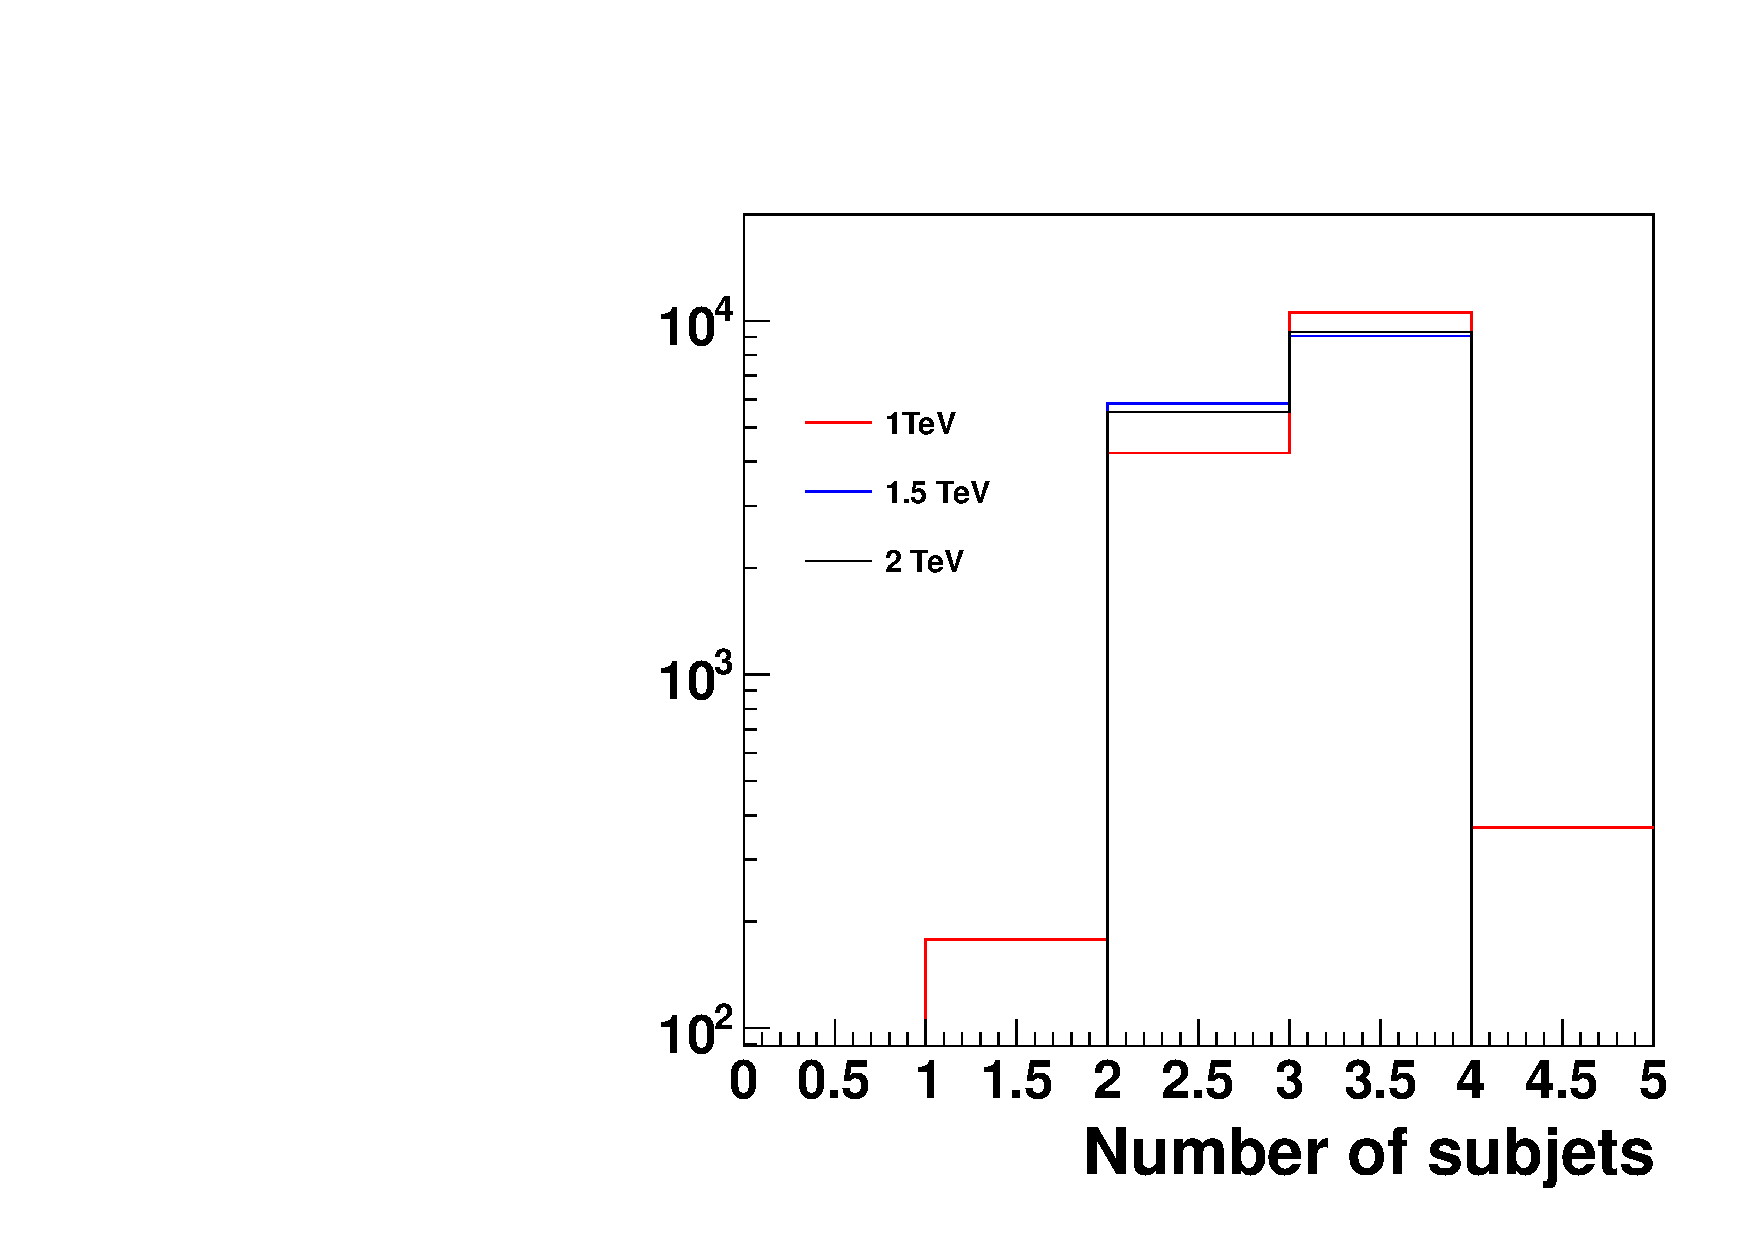
\includegraphics{EXO-14-009/HqqqqZqqfigs/N-subjettiness/Nsubjets.pdf}} 
%     \resizebox{0.5\linewidth}{!}{\includegraphics{HqqqqZqqfigs/N-subjettiness/Tau421TeVAfter.pdf}} \\
\end{tabular}
\caption{Number of subjets of the Higgs jets,  in \HwwVqq signal MC. 
Subjets are abtained from the CMSTopTag jet collection. }
\label{fig:Nsubjets}
\end{figure}


As an alternative, we explore the N-subjettiness, in particular the
variables involving $\tau_4$.  The ratio 
$\tau_{42} \equiv\tau_4/\tau_2$ has the best separation 
between the ${\rm H\to 4q}$
signal and not only QCD background, but also Z and top jets.
Figs~\ref{fig:tau421TeV} and~\ref{fig:tau422TeV} show the
discriminating power of $\tau_{42}$ against $\ttbar$ and QCD, for 1~TeV
and 2~TeV resonance masses respectively.

\begin{figure}[htbp]
  \centering
  \begin{tabular}{cc}
    \resizebox{0.5\linewidth}{!}{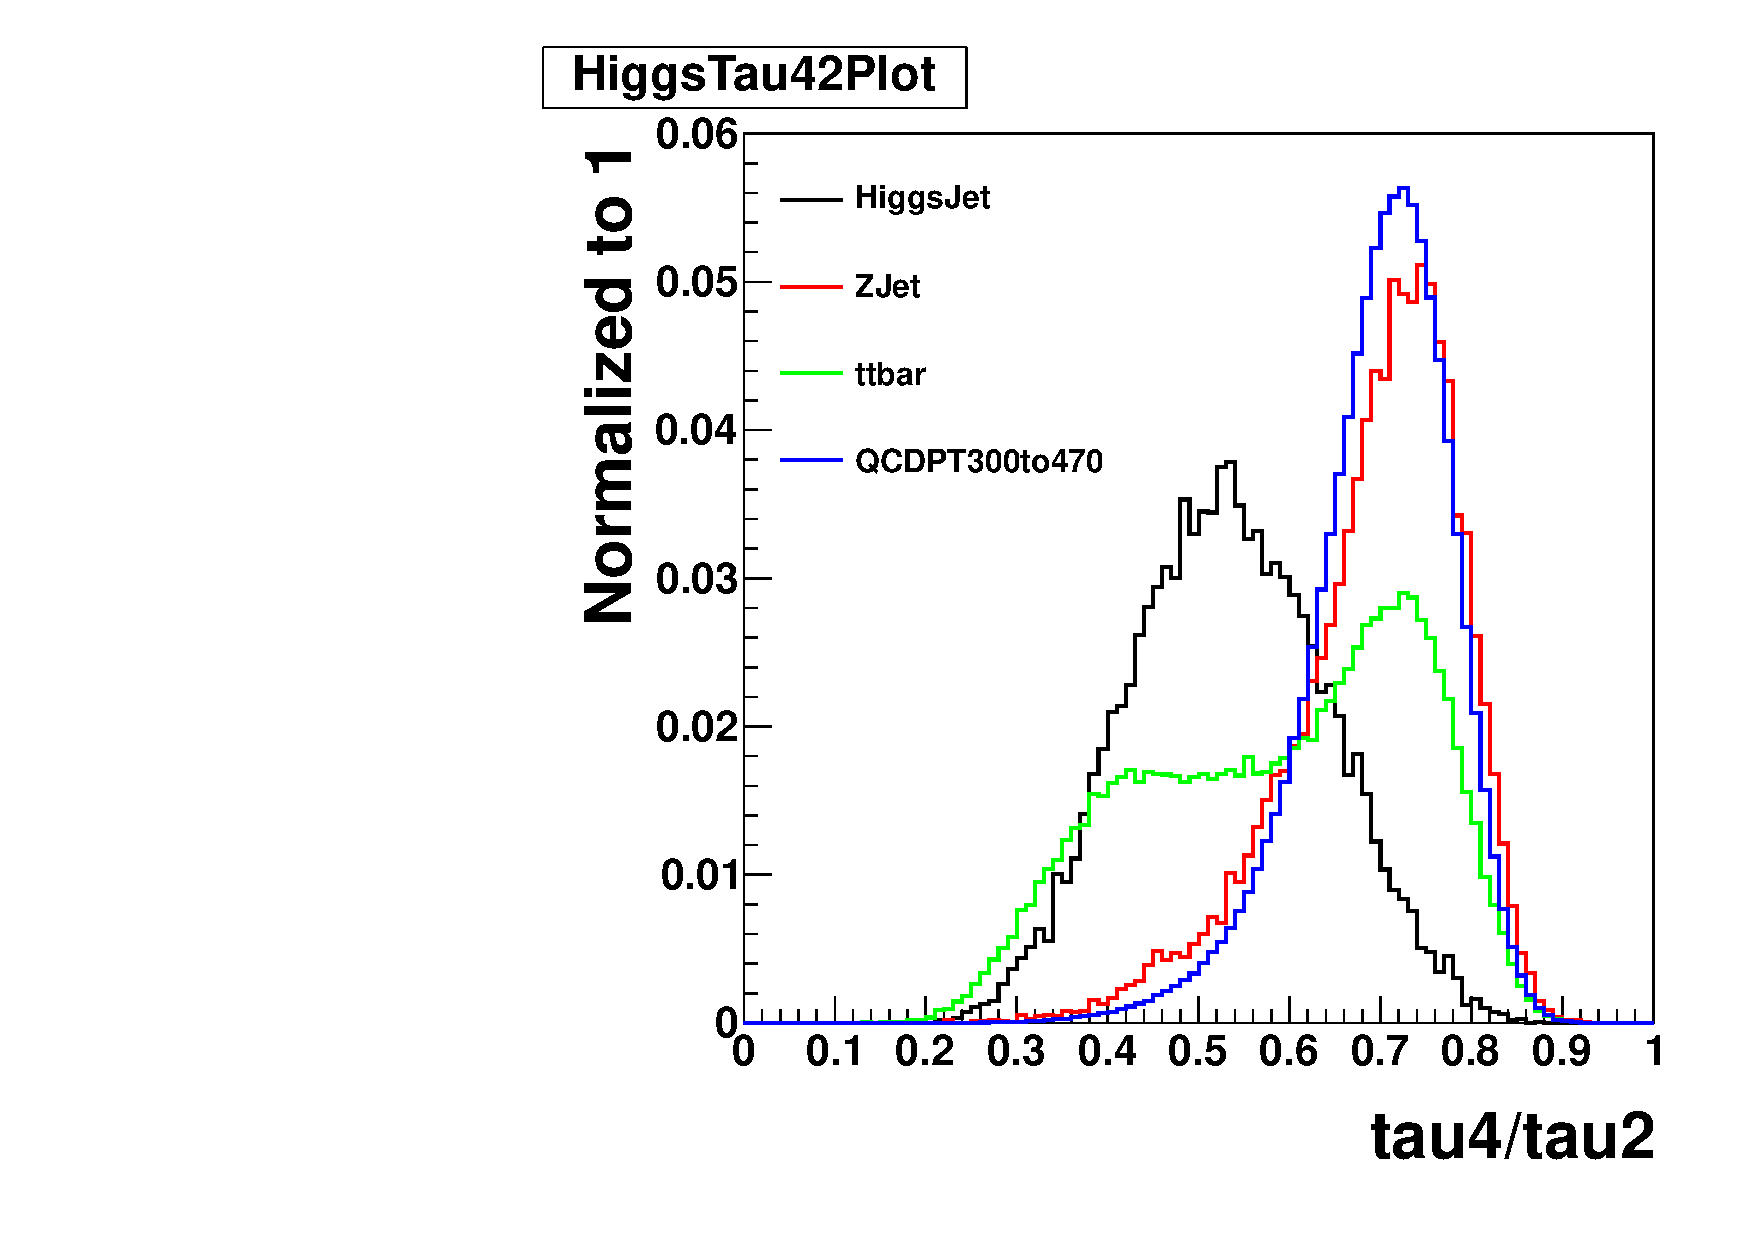
\includegraphics{EXO-14-009/HqqqqZqqfigs/N-subjettiness/Tau421TeVPre.pdf}} &
    \resizebox{0.5\linewidth}{!}{\includegraphics{EXO-14-009/HqqqqZqqfigs/N-subjettiness/Tau421TeVAfter.pdf}} \\
  \end{tabular}
  \caption{ 
    Distribution for $\tau_{4}/\tau_{2}$ in data and in
    simulations of signal (1.0 TeV) and background events.  All simulated
    distributions are scaled to match the number of events in data,
   % except that matched top is scaled to its fraction of unmatched
   %$ ${\rm t\bar{t}}$ times the number of data events.  
    W/Z, matched
    top and Higgs jets are required to match their generator level
    particles, respectively. }
  \label{fig:tau421TeV}
\end{figure}

\begin{figure}[htbp]
  \centering
  \begin{tabular}{cc}
    \resizebox{0.5\linewidth}{!}{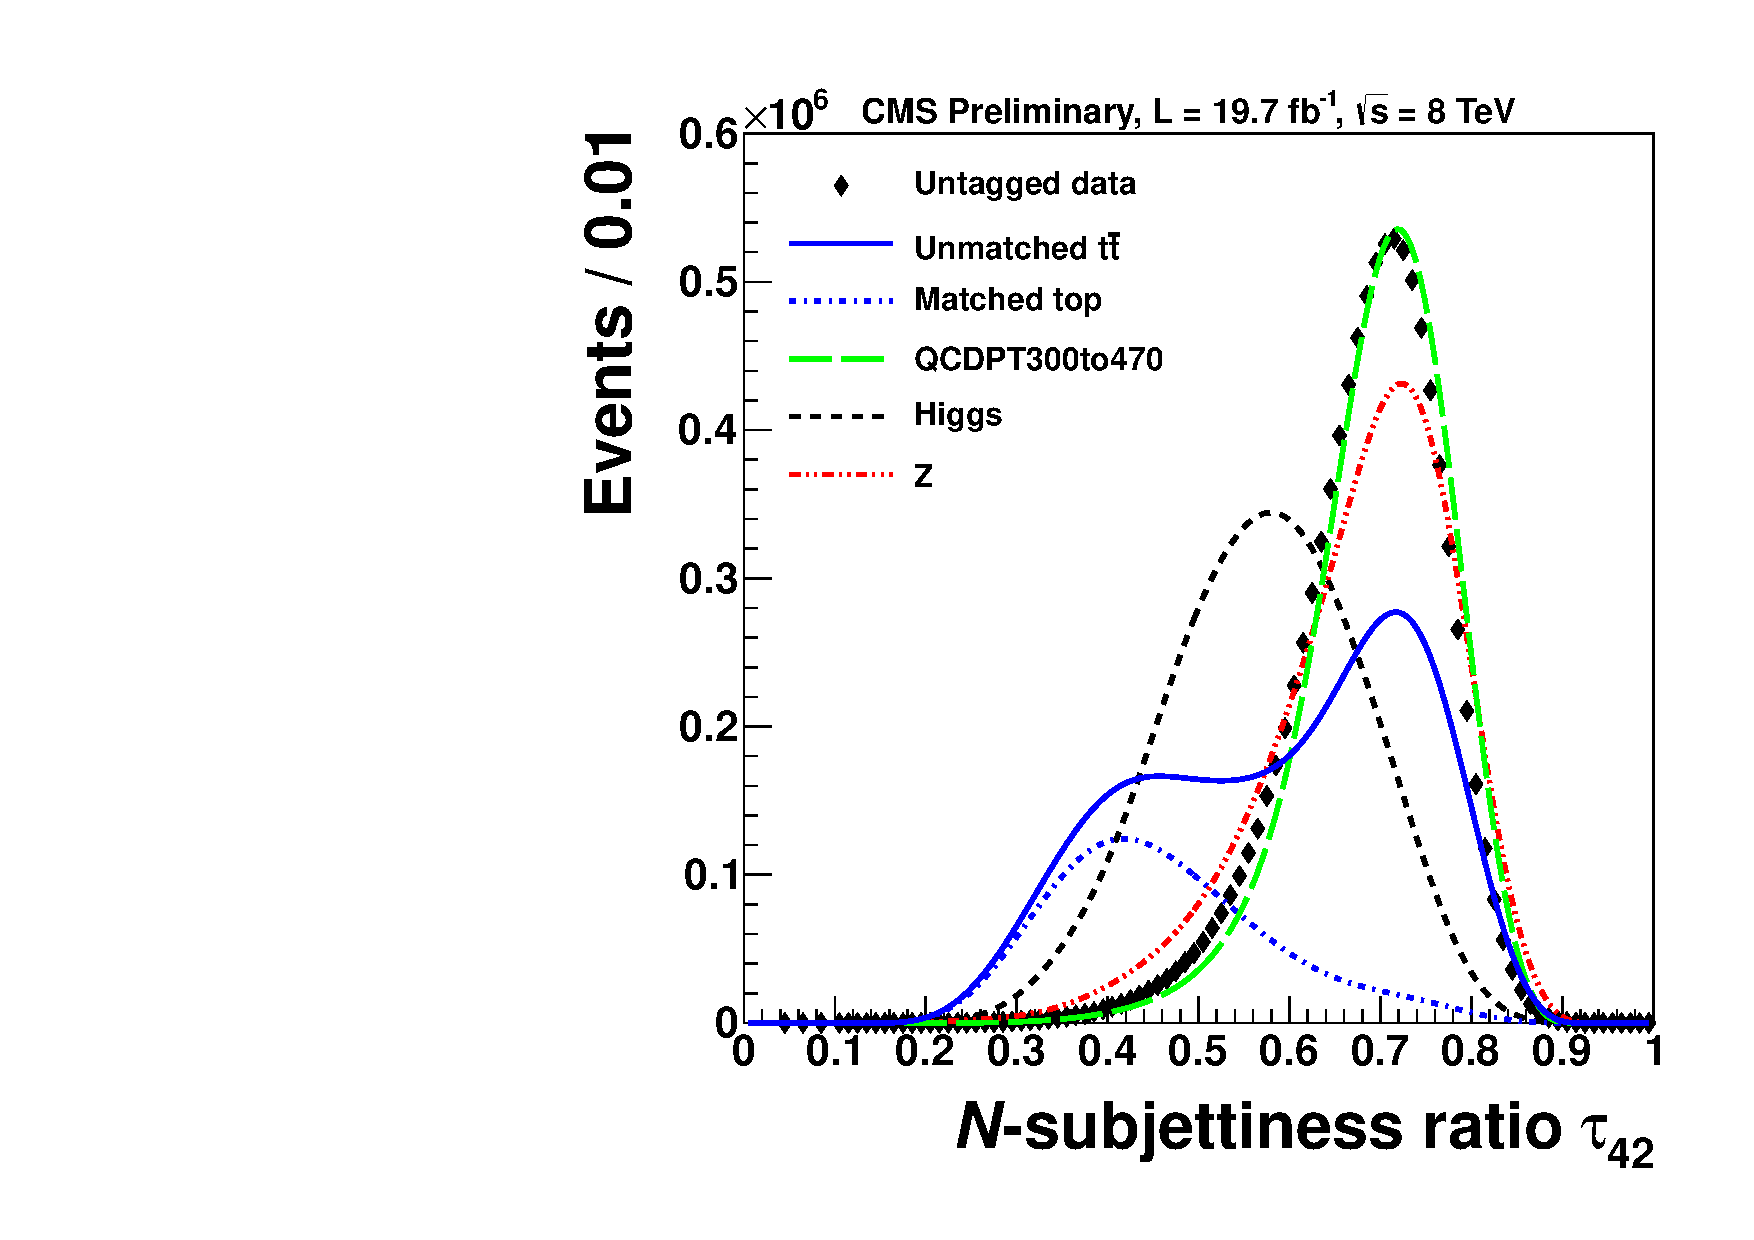
\includegraphics{EXO-14-009/HqqqqZqqfigs/N-subjettiness/tau42PlotAllPre.pdf}} &
    \resizebox{0.5\linewidth}{!}{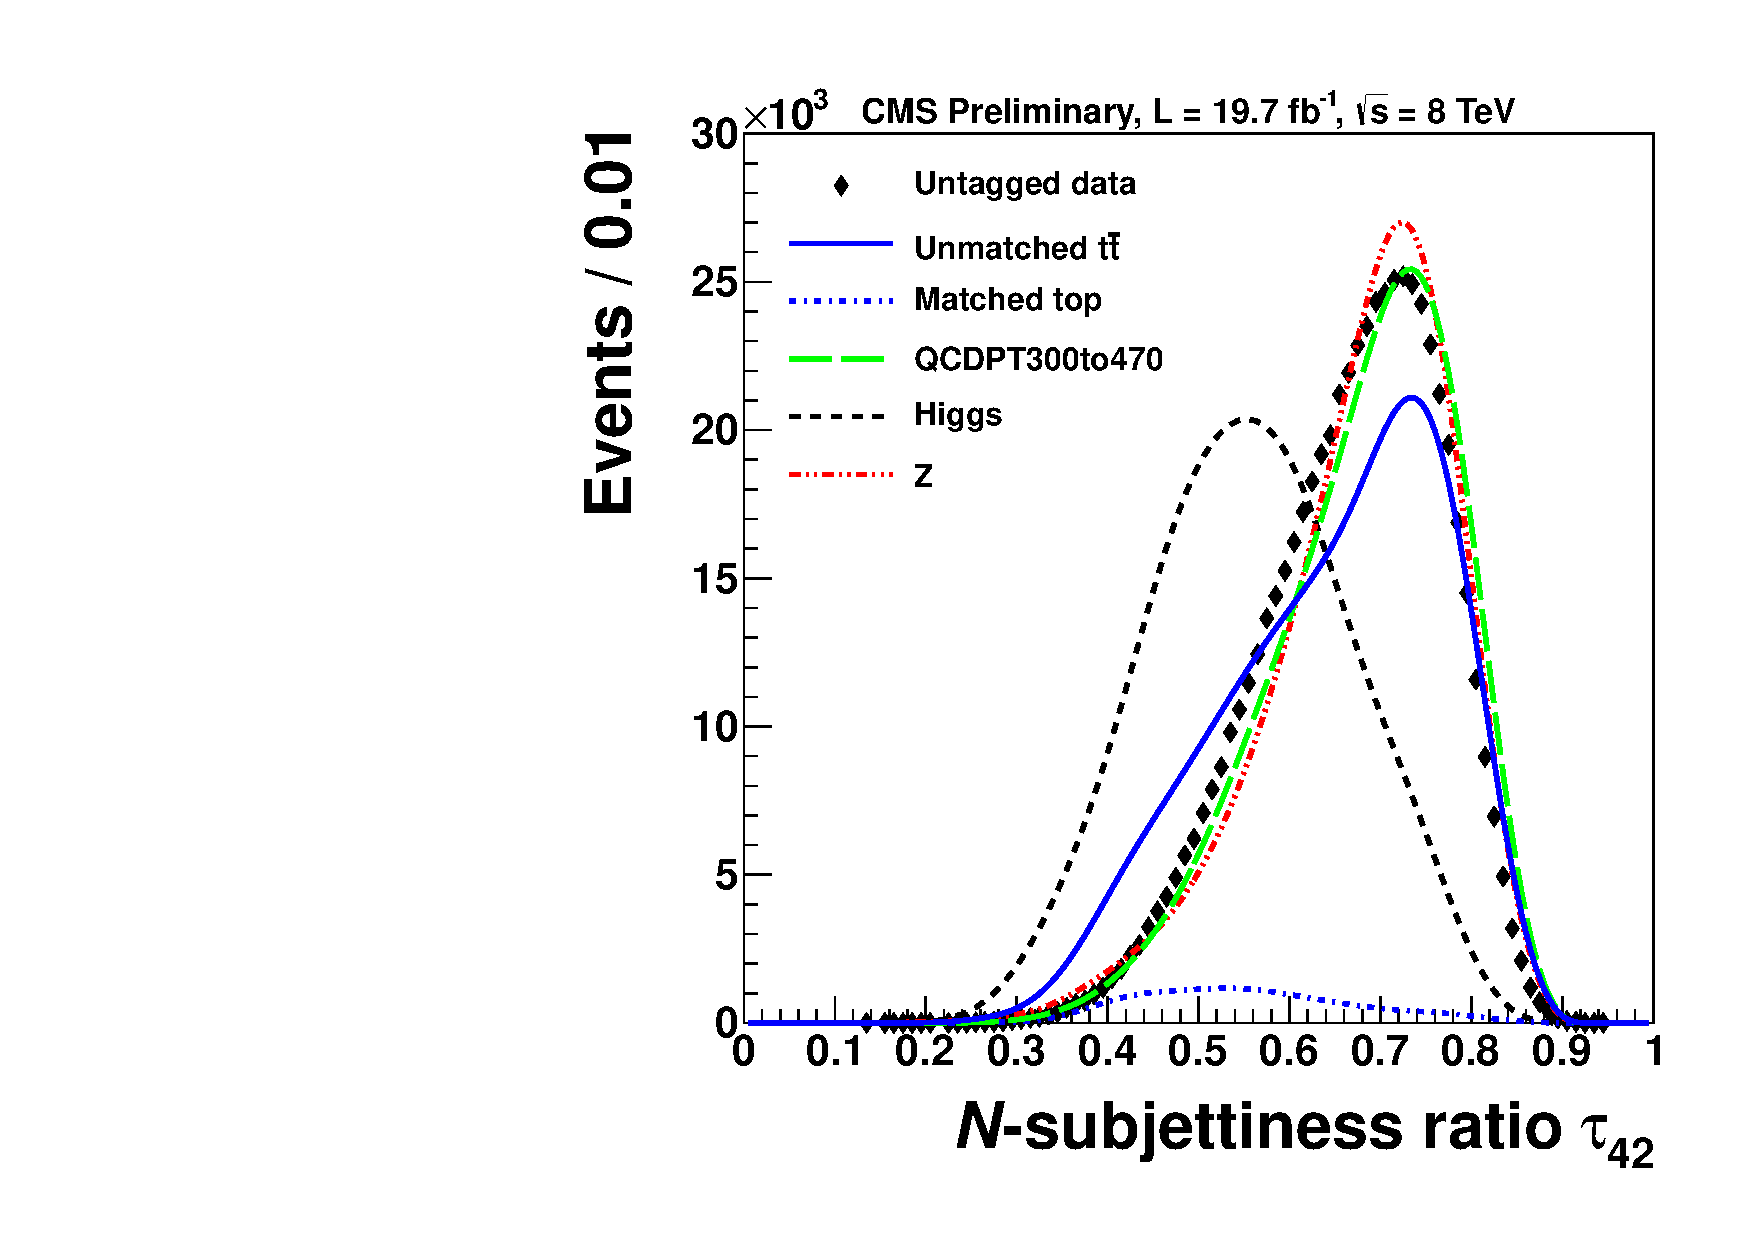
\includegraphics{EXO-14-009/HqqqqZqqfigs/N-subjettiness/tau42PlotAllAfter.pdf}} \\
  \end{tabular}
  \caption{ Distribution for $\tau_{4}/\tau_{2}$ in data and in
    simulations of signal (2.0 TeV) and background events.  All simulated
    distributions are scaled to match the number of events in data,
    except that matched top is scaled to its fraction of unmatched
    ${\rm t\bar{t}}$ times the number of data events.  W/Z, matched
    top and Higgs jets are required to match their generator level
    particles, respectively.  }
  \label{fig:tau422TeV}
\end{figure}

We also explore other combinations of $\tau_{NM} \equiv \tau_N/\tau_M $,
which are listed in Appendix.~\ref{appendix:tauNM}.
The ROC (receiver operating characteristic) 
curve of for several $\tau_{NM}$ cuts (but the same pruned jet mass cut)
is shown in Fig.~\ref{fig:roc}.  The signal efficiency is evaluated
using Higgs jets in 2 \TeVcc signal MC, and the false positive rate
({\it i.e.}, mistag rate) is derived from QCDPT300to470 MC sample.
From the figure, it is clear that $\tau_{42}$ outperforms any other
single $\tau_{NM}$ variable.
%
%
\begin{figure}[htbp]
  \centering
  \begin{tabular}{cc}
    \resizebox{0.7\linewidth}{!}{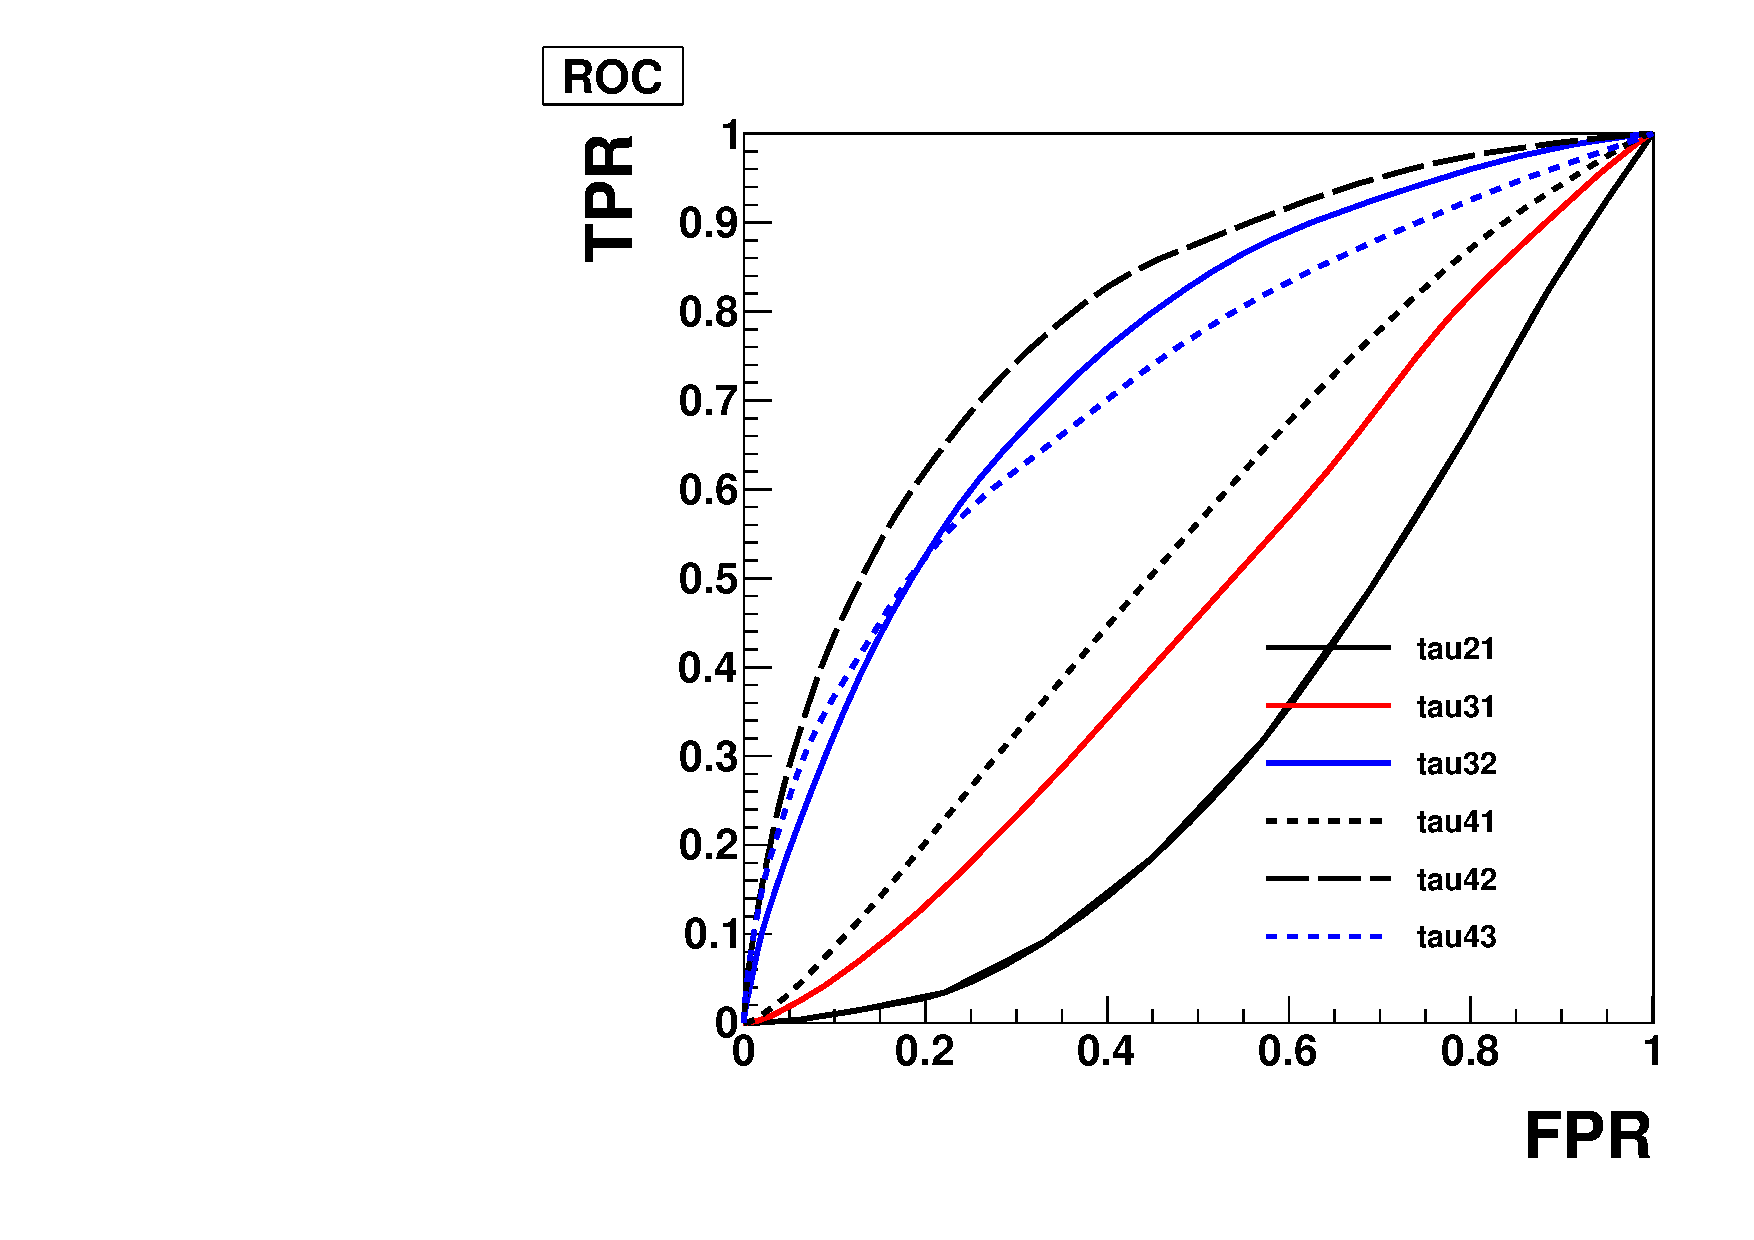
\includegraphics{EXO-14-009/ROC.pdf}} 
    %     \resizebox{0.5\linewidth}{!}{\includegraphics{HqqqqZqqfigs/N-subjettiness/Tau421TeVAfter.pdf}} \\
  \end{tabular}
  \caption{ ROC curves for different $\tau_{NM}$ after the cut on the
    pruned jet mass.  The false positive rate (FPR) is obtained from
    QCDPT300to470 and the true positive rate (TPR) from Higgs jets
    in 2 \TeVcc signal MC sample.  Using $\tau_{42}$ to select Higgs
    jets outperforms all other $\tau_{NM}$ variables. }
  \label{fig:roc}
\end{figure}



After optimizing the cut on $\tau_{42}$ (documented in
Sec.~\ref{sec:tau42Opti} below), the full selection of the ${\rm H \to
  WW^* \to 4q}$ tagger is:
\begin{itemize}

\item {\bf Pruned jet mass}  $\mbox{\boldmath$m_{\text{jet}}$}$
  - We require the total pruned jet mass to satisfy $110 \GeVcc < m_\text{jet} <  135 \GeVcc $.

\item {\bf N-subjettiness}
  - We split the events into two categories, ``high purity'' Higgs jets by
    requiring $\tau_{42} \leq 0.55$, while $ 0.55 < \tau_{42} < 0.65$ defines
    the ``low purity'' Higgs jets.  

\end{itemize}
 



\clearpage

%\subsection{$\tau_4/\tau_2$ optimization study}
\subsubsection{Optimization of the $\tau_4/\tau_2$ threshold}
\label{sec:tau42Opti}


Having selected $\tau_{42}$ as the discriminating variable, we next
optimize its upper value.  In this study, the jet mass is confined
within $[110, 135]~\GeV$.  We use the limit setting method (described
in Sec.~\ref{sec:statistics}) and evaluate the expected limits of
several signal resonance masses at different $\tau_{42}$ working
points.  These expected limits are presented
in Table.~\ref{table:tau42Opti}.
Given our focus on the resonance masses above 1500~\GeVcc, we
choose to cut on $\tau_{42} < 0.55$. In the following analysis, 
to compensate the signal efficiency loss at higher resonance mass, we 
introduce an additional categories for $\Hww$ tagger as $0.55 < \tau_{42} < 0.65$.
This is chosen from back-of-envelope calculation based on 
Figs~\ref{fig:tau421TeV} and~\ref{fig:tau422TeV}, since this category provides 
very limited sensitivity.  
%Figure~\ref{}i 

\begin{table}[htbp]
\begin{center}
\caption{Upper limits (in units of 0.01~pb) 
for high purity HW and HZ signals at different resonance masses and also
different $\tau_{42}$ working points. }
\label{table:tau42Opti}
\begin{tabular}{|r|r|r|r|r|}
\hline
\multicolumn{1}{|l|}{HW / $\tau_{42}$} & 0.45 & 0.5 & 0.55 & 0.6 \\ 
1000 & 4.14 & 4.09 & 4.46 & 4.91 \\ 
1500 & 0.97 & 0.88 & 0.86 & 0.91 \\ 
2000 & 0.89 & 0.64 & 0.51 & 0.47 \\ 
2500 & 1.36 & 0.82 & 0.53 & 0.40 \\ \hline 
\multicolumn{1}{|l|}{HZ / $\tau_{42}$} & \multicolumn{1}{l|}{} & \multicolumn{1}{l|}{} & \multicolumn{1}{l|}{} & \multicolumn{1}{l|}{} \\ 
1000 & 4.31 & 4.36 & 4.63 & 5.05 \\ 
1500 & 0.98 & 0.89 & 0.86 & 0.90 \\ 
2000 & 0.70 & 0.55 & 0.42 & 0.39 \\ 
2500 & 0.96 & 0.61 & 0.41 & 0.32 \\ \hline
\end{tabular}
\end{center}
\end{table}



%\subsection{Summary of Higgs and W/Z tagging categories}
%\label{sec:total}

%In summary, the W or Z jets from the signal are selected by the
%V-tagger, and the Higgs candiadates are selected by an OR of the two
%Higgs taggers, $\Hbb$ and $\Hww$.  Both V-tagger and $\Hww$ taggers 
%have high-purity and
%low-purity categories.  The latter are added to increase the
%sensitivity of the analysis at high resonance masses, where the QCD
%background is low, and a higher signal efficiency is at the premium.
%All the `two-dimensional' categories are shown in
%Table~\ref{table:categories}.  For the \HwwVqq\ channel, we drop the
%low-purity Higgs and low-purity V-tagging category, because it 
%adds only a negligible sensitivity.

%\begin{table}[htb]
%\begin{center}
%  \topcaption{
%    The five event categories used in this analysis.
%    \label{table:categories}}
%\begin{tabular}{ ccc}
%\hline
%$\Hbb$, $\Vqq$ & $\Hww$, $\Vqq$  \\
%\hline
%high-purity V-tag &  high-purity H-tag, high-purity V-tag \\
%low-purity  V-tag &  high-purity H-tag, low purity V-tag\\
%                  &  high-purity V-tag, low purity H-tag\\
%\hline
%\end{tabular}
%\end{center}
%\end{table}




\iffalse

\begin{table}[htbp]
\begin{tabular}{|r|r|r|r|r|r|r|}
\hline
\multicolumn{1}{|l|}{$\tau_{42}$} & \multicolumn{1}{l|}{1000GeV} & \multicolumn{1}{l|}{1500GeV} & \multicolumn{1}{l|}{1800GV} & \multicolumn{1}{l|}{2000GeV} & \multicolumn{1}{l|}{2500GeV} & \multicolumn{1}{l|}{3000GeV} \\ \hline
0.60 & 49.90 & 44.10 & 38.05 & 33.58 & 21.45 & 11.08 \\ \hline
0.55 & 54.20 & 45.33 & 38.52 & 33.91 & 20.88 & 10.69 \\ \hline
0.50 & 55.81 & 45.51 & 37.97 & 32.22 & 19.98 & 9.70 \\ \hline
0.45 & 55.91 & 43.12 & 35.28 & 29.06 & 17.80 & 8.43 \\ \hline
0.40 & 49.17 & 35.99 & 31.21 & 24.55 & 14.13 & 6.73 \\ \hline
0.35 & 37.64 & 28.42 & 22.15 & 18.95 & \multicolumn{1}{l|}{} & \multicolumn{1}{l|}{} \\ \hline
\end{tabular}
\caption{Optimization for $\tau_{42}$ tagger, with a fixed pruned jet 
  mass in $[110~GeV/c^2, 135~GeV/c^2]$.  The table shows the ratio of 
  the number of signal events(without normalization) divided by the number of signal+background
  events(data).}
\label{table:tau42Opti}
\end{table}

\fi



\clearpage

